\begin{dang}{Bài toán tìm m để hàm số có cực trị hoặc đạt cực trị tại điểm cho trước}
	\begin{enumerate}[\iconCV]
		\item Tìm $m$ để hàm số $y=f(x)$ đạt cực trị tại điểm $x_0$ cho trước ($f(x)$ có đạo hàm tại $x_0$):
		\begin{listEX}[1]
			\item [\ding{172}] Giải điều kiện $y'(x_0)=0$, tìm $m$.
			\item [\ding{173}] Lập bảng biến thiên với $m $ vừa tìm được và chọn giá trị $m$ nào thỏa yêu cầu.
				\end{listEX}
	\item Biện luận cực trị hàm số $y=ax^3+bx^2+cx+d$.\\
	Tính $y'=3ax^2+2bx+c$ với $\Delta_{y'}=b^2-3ac$
	\begin{itemize}
		\item[\ding{172}] $\heva{&\Delta_{y'} >0\\&a \ne 0}$: Hàm số có hai điểm cực trị
		\item[\ding{173}]  $\Delta_{y'} \le 0$ hoặc suy biến $\heva{&a=0\\&b=0}$: Hàm số không có cực trị.
	\end{itemize}
	% \begin{note}
		\begin{enumerate}[\iconMT]
				\item Gọi $x_1$, $x_2$ là hai nghiệm phân biệt của $y'=0$ thì $x_1+x_2=-\dfrac{2b}{3a}$ và $x_1\cdot x_2 =\dfrac{c}{3a}$.
			\begin{itemize}
				\item [$\bullet$] $x_1^2+x_2^2=(x_1+x_2)^2-2x_1 x_2$
				\item [$\bullet$] $(x_1-x_2)^2=(x_1+x_2)^2-4x_1 x_2$
				\item [$\bullet$] $x_1^3+x_2^3=(x_1+x_2)^3-3x_1x_2(x_1+x_2)$.
			\end{itemize}
			\item Các công thức tính toán thường gặp:
			\begin{itemize}
				\item [$\bullet$] Độ dài $MN=\sqrt{(x_N-x_M)^2+(y_N-y_M)^2}$
				\item [$\bullet$]  Khoảng cách từ $M$ đến $\Delta$: $d(M,\Delta)=\dfrac{|Ax_M+By_M+C|}{\sqrt{A^2+B^2}}$, với $\Delta \colon Ax+By+C=0$.
				\item [$\bullet$] Tam giác $ABC$ vuông tại $A \Leftrightarrow \overrightarrow{AB} \cdot \overrightarrow{AC}=0 \Leftrightarrow \text{hoành}\cdot\text{hoành}+\text{tung}\cdot\text{tung}=0$.
				\item [$\bullet$] Diện tích tam giác $ABC$ là  $S=\dfrac{1}{2}|a_1b_2-a_2b_1|$, với $\overrightarrow{AB}=(a_1;b_1)$, $\overrightarrow{AC}=(a_2;b_2)$.
			\end{itemize}
			\item PTĐT qua hai điểm cực trị là $y=-\dfrac{2}{9a}(b^2-3ac)x+d-\dfrac{bc}{9a}$.
		\end{enumerate}
	% \end{note}
	\end{enumerate}
\end{dang}
\boxmini{BÀI TẬP TỰ LUẬN}
\setcounter{vd}{0}
\begin{vd}
	Tìm $m$ để hàm số
	\begin{tasks}
		\task  $y=\dfrac{x^3}{3}-mx^2+(m^2-m+1)x+1$ đạt cực tiểu tại $x=3$.
		\task  $y=x^3-3mx^2+3(m^2-1)x$ đạt cực đại tại $x_0=1$.
	\end{tasks}
\loigiai{
\begin{enumerate}[a)]
	\item Ta có $y'=x^2-2mx+m^2-m+1$. Hàm số đạt cực tiểu tại $x=3$ thì
	$$y'(3)=0 \Leftrightarrow 9-6m+m^2-m+1=0 \Leftrightarrow \hoac{&m=2\\&m=5}.$$
	Lập bảng biến thiên của hàm số với lần lượt hai giá trị $m$ vừa tìm được, ta thấy $m=2$ thỏa.\\
	Vậy $m=2$.
	\item Ta có $y'=3x^2-6mx+3(m^2-1)$\\
	Điều kiện cần và đủ để thỏa điều kiện bài toán là
	\begin{eqnarray*}
		\heva{&y'(1)=0 \\&y''(1)<0}
		\Leftrightarrow \heva{&3m^2-6m=0 \\&6-6m<0}
		\Leftrightarrow \heva{&m=0 \vee m=2 \\&m>1}
		\Leftrightarrow m=2.
	\end{eqnarray*}
	Vậy $m=2$ thì thỏa bài toán.
\end{enumerate}}
\end{vd}

\begin{vd}
	Tìm tất cả giá trị của tham số $m$ để hàm số (đồ thị hàm số)
	\begin{tasks}
		\task $ y=x^3-3x^2+2mx+m+2024$ có hai điểm cực trị.
		\task $ y=\dfrac{1}{3}x^3-mx^2+\left(m+2\right)x+2019$ không có cực trị.
		\task $y=x^3-3(m+1)x^2+12mx+2019$ có hai điểm cực trị $x_1,\ x_2$ thỏa mãn $x_1+x_2+2x_1x_2=-8$.
		\task $y=-x^3-3mx^2+m-2$ với $m$ là tham số có hai điểm cực trị $A,B$ sao cho $AB=2$.
	\end{tasks}
\loigiai{
\begin{enumerate}[a)]
	\item Ta có $y’=3x^2-6x+2m$.\\
	Hàm số có cực đại, cực tiểu khi và chỉ khi phương trình $y’=0$ có hai nghiệm phân biệt $\Leftrightarrow {\Delta }’_{y’}>0$ $\Leftrightarrow 9-6m>0$ $\Leftrightarrow m<\dfrac{3}{2}$.
	\item Ta có $y’=x^2-2mx+m+2$\\
	Hàm số đã cho không có cực trị $\Leftrightarrow$ phương trình $y’=0$ vô nghiệm hoặc có nghiệm kép hay ${\Delta }’_{y’} \le 0$ $\Leftrightarrow m^2-\left( m+2 \right)\le 0$ $\Leftrightarrow -1\le m\le 2$.
	\item Ta có $y'=3x^2-6(m+1)x+12m,\ y'=0\Leftrightarrow 3x^2-6(m+1)x+12m=0$. \\
	Hàm số có hai điểm cực trị $\Leftrightarrow \Delta '=9m^2-18m+9>0\Leftrightarrow m\ne 1$.\tagEX{1}
	Giả sử $x_1,\ x_2$ là hai nghiệm của phương trình $y'=0$, theo định lí Vi-ét ta có
	$$\heva{&x_1+x_2=-\dfrac{b}{a}=2(m+1)\\&x_1\cdot x_2=\dfrac{c}{a}=4m.}$$
	Do đó $x_1+x_2+2x_1\cdot x_2=-8\Leftrightarrow 2(m+1)+8m=-8\Leftrightarrow 10m=-10\Leftrightarrow m=-1$ thỏa mãn $(1)$.\\
	Vậy $m=-1$ là giá trị cần tìm của $m$.
	\item Ta có $y'=-3x^2-6mx$; $y'=0\Leftrightarrow
	\hoac{&x=0\\&x=-2m.\\}$\\
	Hàm số có hai điểm cực trị khi và chỉ khi $m\ne 0$.\\
	Gọi hai điểm cực trị của đồ thị hàm số là $A$, $B$.\\
	Ta có $A\left(0;m-2\right)$, $ B\left(-2m;-4{m}^{3}+m-2\right)$.\\
	Do đó
	{\allowdisplaybreaks
		\begin{align*}
			AB^2=4m^2+16m^6=4&\Leftrightarrow 4m^6+m^2-1=0\\
			&\Leftrightarrow m^2=\dfrac{1}{2}\Leftrightarrow m=\pm \dfrac{1}{\sqrt{2}}.
	\end{align*}}
\end{enumerate}}
\end{vd}

\boxmini{BÀI TẬP TRẮC NGHIỆM}
\ind{PHẦN I.} \inden{Câu trắc nghiệm nhiều phương án lựa chọn. Mỗi câu hỏi học sinh chỉ chọn một phương án.}\\
\setcounter{ex}{0}
\Opensolutionfile{ans}[ans/2D1-B1-d3-1]

\begin{ex}
	Tìm tất cả giá trị của tham số $m$ để hàm số $y=\dfrac{1}{3}x^3+(m+1)x^2+(1-3m)x+2$ có cực đại và cực tiểu.
	\choice
	{$m\leq-5;m\geq 0$}
	{\True $m <-5$; $m>0$}
	{$-5<m<0$}
	{$-5\leq m\leq 0$}
	\loigiai{
		Tập xác định $\mathscr{D}=\mathbb{R}$.\\
		Ta có $y’=x^2+2(m+1)x+1-3m$.\\
		Hàm số có cực đại và cực tiểu khi phương trình $y’=0$ có hai nghiệm phân biệt và đổi dấu qua các nghiệm đó.\\
		Khi đó $\Delta’_{y’}=(m+1)^2-(1-3m)>0\Leftrightarrow m^2+5m>0\Leftrightarrow \hoac{&m<-5\\&m>0.}$}
\end{ex} 

\begin{ex}
	Tìm tất cả các giá trị của tham số $ m $ để hàm số $ y=-x^3-3x^2+mx+2 $ có cực đại và cực tiểu.
	\choice
	{\True $m>-3$}
	{$m\geq 3$}
	{$m\geq-3$}
	{$m>3$}
	\loigiai{
		Ta có $ y'=-3x^2-6x+m $. Hàm số đã cho có cực đại và cực tiểu khi và chỉ khi phương trình $ y'=0 $ có $ 2 $ nghiệm phân biệt $\Leftrightarrow\Delta'>0\Leftrightarrow 9+3m>0\Leftrightarrow m>-3 $.
	}
\end{ex} 

\begin{ex}
	Cho hàm số $y=x^3-3(m+1)x^2+3(7m-3)x$. Số giá trị nguyên của tham số $m$ để hàm số không có cực trị là
	\choice
	{$2$}
	{$1$}
	{\True $4$}
	{$3$}
	\loigiai{
		Hàm số bậc $3$ không có cực trị khi và chỉ khi phương trình $y'=0 \Leftrightarrow 3x^2-6(m+1)x+3(7m-3)=0$ có nghiệm kép hoặc vô nghiệm hay
		$$\Delta' \le 0 \Leftrightarrow 9(m+1)^2-9(7m-3)\le 0 \Leftrightarrow m^2-5m+4 \le 0 \Leftrightarrow 1 \le m \le 4.$$
		Mà $m \in \mathbb{Z}$ nên $ m \in \{1;2;3;4\}$.\\
		Vậy có $4$ giá trị nguyên của $m$ thỏa mãn yêu cầu bài toán.
	}
\end{ex} 

\begin{ex}
	Cho hàm số $y=x^3-3(m+1)x^2+3(7m-3)x$. Gọi $S$ là tập hợp tất cả các giá trị nguyên của tham số $m$ để hàm số không có cực trị. Số phần tử của $S$ là
	\choice
	{$2$}
	{\True $4$}
	{$0$}
	{Vô số}
	\loigiai{
		Tập xác định là $\mathscr{D}=\mathbb{R}$.\\
		$y'=3x^2-6(m+1)x+3(7m-3)$.\\
		Hàm số không có cực trị khi và chỉ khi $\Delta'=9(m+1)^2-9(7m-3)\le 0\Leftrightarrow m^2-5m+4\le 0\Leftrightarrow 1\le m \le 4.$\\
		Vậy có $m\in \{1;2;3;4\}$.
	}
\end{ex} 

\begin{ex}
	Giả sử hàm số $ y=\dfrac{1}{3}x^3-x^2-\dfrac{1}{3}mx$ có hai điểm cực trị $x_1, x_2$ thỏa mãn $x_1+ x_2+2x_1x_2=0$. Giá trị của $ m$ là
	\choice
	{$ m=\dfrac{4}{3}$}
	{$ m=-3$}
	{\True $ m=3$}
	{$ m=2$}
	\loigiai{
		Ta có $y’=x^2-2x-\dfrac{1}{3}m$.\\
		$y’=0\Leftrightarrow  3x^2-6x-m=0$.\\
		Hàm số có hai cực trị $\Leftrightarrow y'=0$ có hai nghiệm phân biệt $\Leftrightarrow 9+3m>0 \Leftrightarrow m>-3$.\\
		Khi đó $x_1+ x_2 + 2x_1x_2=0 \Leftrightarrow 2-\dfrac{2m}{3}=0 \Leftrightarrow m=3$ (TM).}
\end{ex} 

\begin{ex}
	Cho hàm số $ f\left( x \right)=x^3-3x^2+mx-1$. Tìm giá trị của tham số $m$ để hàm số có hai cực trị $x_1, x_2$ thỏa $x_1^2+x_2^2=3$.
	\choice
	{$ m=\dfrac{1}{2}$}
	{$ m=-2$}
	{$ m=1$}
	{\True $ m=\dfrac{3}{2}$}
	\loigiai{
		TXĐ $D=\mathbb{R}$.\\
		${f}’\left( x \right)=3x^2-6x+m$.\\
		Hàm số có hai điểm cực trị $x_1, x_2 \Leftrightarrow {f}’\left( x \right)=0$ có hai nghiệm phân biệt $\Leftrightarrow 9-3m>0  \Leftrightarrow m<3$.\\
		Theo hệ thức Vi-et: $x_1+ x_2=2$; $x_1.x_2=\dfrac{m}{3}$.\\
		Khi đó: $x_1^2+x_2^2=3  \Leftrightarrow  \left( {x_1+ x_2} \right)^2 - 2x_1x_2=3 \Leftrightarrow 2^2-\dfrac{2m}{3}=3 \Leftrightarrow m=\dfrac{3}{2}$.}
\end{ex} 

\begin{ex}
	Tìm tất cả các giá trị của tham số $m$ để đồ thị hàm số $y=x^3-12x+m+2$ có hai cực trị và hai điểm cực
	trị này nằm về hai phía trục hoành?
	\choice
	{$m=-2$}
	{\True $-18<m<14$}
	{$\forall m\in \mathbb{R}$}
	{$m\neq 1$}
	\loigiai{
		Ta có $y'=3x^2-12$. Suy ra $y'=0\Leftrightarrow \hoac{& x=2\Rightarrow y=m-14 \\ & x=-2\Rightarrow y=m+18.}$\\
		Đồ thị hàm số có hai điểm cực trị nằm về hai phía trục hoành khi và chỉ khi
		$$(m-14)(m+18)<0\Leftrightarrow -18<m<14.$$
	}
\end{ex} 

\begin{ex}
	Tập hợp các giá trị của $m$ để đồ thị hàm số $y=x^3+mx^2-\left(m^2-4\right)x+1$ có hai điểm cực trị nằm ở hai phía của trục $Oy$ là
	\choice
	{$(-\infty;2)$}
	{\True $\mathbb{R}\setminus[-2;2]$}
	{$(-2;2)$}
	{$(2;+\infty)$}
	\loigiai{
		Ta có $y'=3x^2+2mx+4-m^2$.\\
		Đồ thị hàm số có hai cực trị nằm hai phía đối với trục $Oy$ khi và chỉ khi $y'=0$ có hai nghiệm trái dấu $\Leftrightarrow P=\dfrac{4-m^2}{3}<0\Leftrightarrow\hoac{&m>2\\&m<-2.}$}
\end{ex} 

\begin{ex}
	Cho hàm số $y=x^3+3mx^2+3(m^2-1)x+m^3.$ Tìm $m$ để hàm số đạt cực tiểu tại điểm $x=0.$
	\choice
	{$m=-1$}
	{\True $m=1$}
	{$m=0$}
	{$m=2$}
	\loigiai{
		Ta có $y'=3x^2+6mx+3(m^2-1)$ và $y''=6x+6m\Rightarrow y''(0)=6m.$\\
		Hàm số đạt cực tiểu tại $x=0\Rightarrow y'(0)=0\Leftrightarrow 3(m^2-1)=0\Leftrightarrow m=\pm 1.$\\
		Với $m=1\Rightarrow y''(0)=6>0\Rightarrow$  hàm số đạt cực tiểu tại $x=0.$\\
		Với $m=-1\Rightarrow y''(0)=-6<0\Rightarrow$  hàm số đạt cực đại tại $x=0.$\\
		Vậy $m=1$ thỏa mãn bài.
	}
\end{ex} 

\begin{ex}
	Hàm số $ y=x^3-2mx^2+m^2x-2 $ đạt cực tiểu tại $ x=1 $ khi
	\choice
	{$ m=3 $}
	{$ m=-3 $}
	{\True $ m=1 $}
	{$ m=-1 $}
	\loigiai{
		Ta có: $ y'=3x^2-4mx+m^2 ,
		y''=6x-4m. $\\
		Hàm số đạt cực tiểu tại $ x=1 $, suy ra $y'(1)=0\Leftrightarrow m^2-4m+3=0 \Leftrightarrow \hoac{&m=1\\&m=3.}$
		\begin{itemize}
			\item Với $m=1$ ta có $y'(1)=0, y''(1)=2>0$ nên hàm số đạt cực tiểu tại $x=1$.
			\item Với $m=3$ ta có $y'(1)=0, y''(1)=-6<0$ nên hàm số đạt cực đại tại $x=1$.
	\end{itemize}}
\end{ex} 

\begin{ex}
	Tìm giá trị thực của tham số $m$ để hàm số $y=\dfrac{1}{3}x^3-mx^2+(m^2-4)x+3$ đạt cực tiểu tại $x=3$.
	\choice
	{$m=-1$}
	{\True $m=1$}
	{$m=-7$}
	{$m=5$}
	\loigiai{
		Ta có $y'=x^2-2mx+m^2-4$ và $y''=2x-2m$.\\
		Hàm số đạt cực tiểu tại $x=3$ nên $y'(3)=0 \Leftrightarrow 9-6m+m^2-4=0 \Leftrightarrow \hoac{&m=5 \\ &m=1.}$\\
		Với $m=5$ thì $y''(3)=-4<0$, loại.\\
		Với $m=1$ thì $y''(3)=4>0$, thỏa mãn.
	}
\end{ex} 

\begin{ex}
	Đồ thị hàm số $y=x^3-3x^2+2ax+b$ (với $a, b \in \mathbb{R}$) có điểm cực tiểu $A(2;-2)$. Khi đó $a+b$ bằng
	\choice
	{$-4$}
	{$4$}
	{\True $2$}
	{$-2$}
	\loigiai{
		Ta có: $y’=3x^2-6x+2a; y''=6x-6$.\\
		Đồ thị hàm số có điểm cực tiểu $A(2;-2)$ nên ta có:
		$\heva{&y’(2)=0\\&y(2)=-2} \Leftrightarrow \heva{&2a=0\\&4a+b=2} \Leftrightarrow \heva{&a=0\\&b=2.}$\\
		Với $a=2,b=0$ ta thấy $y''(2)=6.2-6=6>0$ nên hàm số đạt cực tiểu tại $x=2$, thỏa yêu cầu bài toán.\\
		Suy ra $a+b=2$.
	}
\end{ex} 

\begin{ex}
	Gọi $m_1, m_2$ là các giá trị của tham số $m$ để đồ thị hàm số $y=2x^{3}-3x^{2}+m-1$ có hai điểm cực trị $B, C$ sao cho tam giác $OBC$ có diện tích bằng 2, với $O$ là gốc tọa độ. Tích $m_{1} \cdot m_{2}$ bằng
	\choice
	{$12$}
	{$6$}
	{\True $-15$}
	{$-20$}
	\loigiai{
		Tập xác định: $\mathscr{D}=\mathbb{R}$.\\
		Ta có \begin{eqnarray*}
			y'=6 x^{2}-6 x=0 &\Leftrightarrow&
			\hoac{x=0 \Rightarrow y=m-1 \Rightarrow B(0 ; m-1) \\ x=1 \Rightarrow y=m-2 \Rightarrow C(1 ; m-2)}\\
			&\Rightarrow& S_{\triangle OBC}=\dfrac{1}{2} d(C ; O B) \cdot O B=\dfrac{1}{2} \cdot 1 \cdot |m-1|=2\\
			&\Leftrightarrow& |m-1|=4
			\Leftrightarrow \hoac{&m_1=5 \\ &m_2=-3.}
		\end{eqnarray*}
		Vậy $m_1 \cdot m_2 = -15$.
	}
\end{ex} 

\begin{ex}
	Cho hàm số $y=x^3-3mx^2+3m^3$. Biết rằng có hai giá trị của tham số $m$ để đồ thị hàm số có hai điểm cực trị $A,B$ và tam giác $OAB$ có diện tích bằng $48$. Khi đó tổng các giá trị của $m$ là
	\choice
	{\True $0$}
	{$2$}
	{$\sqrt{2}$}
	{$-2$}
	\loigiai{
		Tập xác định $\mathscr{D}=\mathbb{R}$.\\
		Đạo hàm $y'=3x^2-6mx$, xác định với mọi $x\in\mathbb{R}$.\\
		$y'=0\Leftrightarrow\hoac{&x=0\\&x=2m.}$ \\
		Do đó hàm số có hai cực trị khi và chỉ khi $m\neq 0$.\\
		Khi đó $A\left(0;3m^3\right)$, $B\left(2m;-m^3\right)$.\\
		Suy ra $\overrightarrow{OA}=\left(0;3m^3\right)$, $\overrightarrow{OB}=\left(2m;-m^3\right)$.\\
		$S_{\triangle OAB}=48\Leftrightarrow \dfrac{1}{2}\left|\left[\overrightarrow{OA},\overrightarrow{OB}\right]\right|=48\Leftrightarrow \left|-6m^4\right|=96\Leftrightarrow m=\pm 2$.\\
		Vậy tổng các giá trị của $m$ là $0$.
	}
\end{ex} 
\Closesolutionfile{ans}

\ind{PHẦN II.} \inden{Câu trắc nghiệm đúng sai. Trong mỗi ý a), b), c), d) ở mỗi câu, học sinh chọn đúng hoặc sai.}\\
\Opensolutionfile{ans}[ans/2D1-B1-d3-2]

\begin{ex}
	Cho hàm số $ y=\dfrac{m}{3}x^3+2x^2+mx+1$, với $m$ là tham số.
	\choiceTF
	{Hàm số có hai điểm cực trị khi $-2<m<2$}
	{Hàm số có đúng một điểm cực trị khi $m=0$ hoặc $m=2$}
	{\True Hàm số không có cực trị khi $m \le -2$ hoặc $m \ge 2$}
	{\True Hàm số có $2$ điểm cực trị thỏa mãn $x_\text{CĐ}<x_{CT}$ khi $0<m<2$}
	\loigiai{
		\begin{enumerate}[a)]
			\item Ta có $y’=mx^2+4x+m$.\\
			Hàm số có $2$ điểm cực trị $\Leftrightarrow y’=0$ có $2$ nghiệm phân biệt $\Leftrightarrow \left\{ \begin{aligned}
				& m\ne 0 \\
				& 4-m^2>0 \\
			\end{aligned} \right.\Leftrightarrow \left\{ \begin{aligned}
				& m\ne 0 \\
				& -2<m<2 \\
			\end{aligned} \right.\quad(1)$.
			\item Hàm số có đúng 1 cực trị khi hàm số này bị suy biến về hàm bậc hai, nghĩa là $\dfrac{m}{3}=0 \Leftrightarrow m=0$.
			\item Với $m=0$ thì hàm số trở thành $y=2x^2+1$. Hàm số này có 1 điểm cực tiểu. Điều này không thỏa yêu cầu bài toán\\
			Với $m \ne 0$: Hàm số không có cực trị $\Leftrightarrow y’=0$ có vô nghiệm hoặc nghiệm kép. $\Leftrightarrow \left\{ \begin{aligned}
				& m\ne 0 \\
				& 4-m^2 \le 0 \\
			\end{aligned} \right.\Leftrightarrow \left\{ \begin{aligned}
				& m\ne 0 \\
				&  m \le -2,\,m \ge 2\\
			\end{aligned} \right.$.
			\item Dựa vào dạng đồ thị hàm số bậc $3$, hàm số có $2$ điểm cực trị thỏa mãn $x_\text{CĐ}<x_{CT}$ khi $ m>0$ $(2)$\\
			Từ $\left(1\right)$ và $\left(2\right)$ suy ra giá trị $ m$ cần tìm là $0<m<2$.
		\end{enumerate}
}
\end{ex} 

\begin{ex}
	Cho hàm số $y=x^3-3mx^2+3\left(m^2-1\right)x-m^3$ với $m$ là tham số.
	\choiceTF
	{\True Hàm số luôn có hai điểm cực trị với mọi $m$}
	{\True Hàm số đạt cực tiểu tại $x=3$ khi $m=2$}
	{\True Khi đồ thị hàm số có hai điểm cực trị thì khoảng cách giữa hai điểm cực trị bằng $2\sqrt{5}$}
	{\True Điểm cực tiểu của đồ thị hàm số luôn thuộc đường thẳng cố định với hệ số góc $k=-3$}
	\loigiai
	{
		\begin{enumerate}[a)]
			\item Ta có $y'=3x^2-6mx+3\left(m^2-1\right). y'=0\Leftrightarrow \hoac{&x_1=m-1\\&x_2=m+1}$.\\
			Do $x_1 \ne x_2, \,\forall m$ nên hàm số luôn có hai điểm cực trị.
			\item Dễ thấy $x=m+1$ là điểm cực tiểu. Suy ra, hàm số đạt cực tiểu tại $x=3$ khi $m+1=3 \Leftrightarrow m=2$.
			\item Với mọi $m$, tọa độ hai điểm cực trị là $A(m+1;-3m-2)$ và $B(m-1;-3m+2)$.\\
			Khoảng cách giữa hai điểm cực trị là $AB=\sqrt{(x_B-x_A)^2+(y_B-y_A)^2}=2\sqrt{5}$.
			\item Ta có $y'=3x^2-6mx+3\left(m^2-1\right). y'=0\Leftrightarrow \hoac{&x=m-1\\&x=m+1}$\\
			Vì là hàm số bậc ba với hệ số $a=1>0$ nên điểm cực tiểu của hàm số là $A\left(m+1;-3m-2\right)$. \\
			Lại có $-3m-2=-3\left(m+1\right)+1$ nên điểm cực tiểu của hàm số luôn thuộc đường thẳng $d:y=-3x+1$, hệ số góc $k=-3$.
		\end{enumerate}
	}
\end{ex} 

\begin{ex}
	Cho hàm số $y=\dfrac{x^2-2mx +m +2}{x-m}$, với $m$ là tham số.
	\choiceTF
	{\True Tập xác định của hàm số là $\mathbb{R}\backslash\{m\}$}
	{\True Có hai giá trị nguyên của tham số $m$ để hàm số có hai điểm cực trị}
	{\True Hàm số đạt cực đại tại $x=-1$ khi $m=\dfrac{1}{2}$}
	{Khi đồ thị hàm số có hai điểm cực trị thì đường thẳng qua hai điểm cực trị của đồ thị có phương trình là $y=2x-2m$}
	\loigiai{
		\begin{enumerate}[a)]
			\item Hàm số xác định khi $x-m \ne 0 \Leftrightarrow x \ne m$. Suy ra $\mathscr{D}=\mathbb{R}\backslash\{m\}$.
			\item $y'=\dfrac{x^2-2mx+2m^2-m-2}{(x-m)^2}$.\\
			Để hàm số có hai điểm cực trị thì $y'=0$ có hai nghiệm phân biệt khác $m$ hay $g(x)=x^2-2mx+2m^2-m-2$ có hai nghiệm phân biệt khác $m$.
			$$\Leftrightarrow \heva{&\Delta'>0\\&g(m) \ne 0} \Leftrightarrow \heva{&-m^2+m+2>0\\&m^2-m-2 \ne 0}  \Leftrightarrow m \in (-1;2).$$
			Vì $m$ nguyên nên $m \in \{0;1\}$.
			\item Hàm số đạt cực trị tại $x=-1$ thì $y'(-1)=0 \Leftrightarrow 2m^2+m-1 =0 \Leftrightarrow m=-1$ hoặc $m=\dfrac{1}{2}$.\\
			Thử lại với $m=\dfrac{1}{2}$, ta có $y'=\dfrac{x^2-x-2}{x-\dfrac{1}{2}}$.\\
				Bảng biến thiên
				\begin{center}
					\begin{tikzpicture}
						\tkzTabInit[nocadre=false,lgt=1,espcl=3]
						{$x$ /0.7,$y'$ /0.7,$y$ /2}
						{$-\infty$,$-1$,$0.5$,$2$,$+\infty$}
						\tkzTabLine{,+,$0$,-,d,-,$0$,+,}
						\tkzTabVar{-/$-\infty$,+/$y_1$,-D+/$-\infty$/$+\infty$,-/$y_2$,+/$+\infty$}
					\end{tikzpicture}
				\end{center}
			Suy ra $m=\dfrac{1}{2}$ thỏa yêu cầu bài toán.
			\item Cho hàm số $y=\dfrac{u(x)}{v(x)}$. Nếu đồ thị hàm số có hai điểm cực trị thì đường thẳng qua hai điểm cực trị có dạng $y=\dfrac{u'(x)}{v'(x)}$.\\
			Áp dụng, ta được $y=\dfrac{(x^2-2mx+m+2)'}{(x-m)'}=2x-2m$
		\end{enumerate}
	}
\end{ex} 

\Closesolutionfile{ans}
